
%% bare_conf.tex
%% V1.4a
%% 2014/09/17
%% by Michael Shell
%% See:
%% this can cause conflict
%% http://www.michaelshell.org/
%% for current contact information.
%%
%% This is a skeleton file demonstrating the use of IEEEtran.cls
%% (requires IEEEtran.cls version 1.8a or later) with an IEEE
%% conference paper.
%%
%% Support sites:
%% http://www.michaelshell.org/tex/ieeetran/
%% http://www.ctan.org/tex-archive/macros/latex/contrib/IEEEtran/
%% and
%% http://www.ieee.org/

%%*************************************************************************
%% Legal Notice:
%% This code is offered as-is without any warranty either expressed or
%% implied; without even the implied warranty of MERCHANTABILITY or
%% FITNESS FOR A PARTICULAR PURPOSE! 
%% User assumes all risk.
%% In no event shall IEEE or any contributor to this code be liable for
%% any damages or losses, including, but not limited to, incidental,
%% consequential, or any other damages, resulting from the use or misuse
%% of any information contained here.
%%
%% All comments are the opinions of their respective authors and are not
%% necessarily endorsed by the IEEE.
%%
%% This work is distributed under the LaTeX Project Public License (LPPL)
%% ( http://www.latex-project.org/ ) version 1.3, and may be freely used,
%% distributed and modified. A copy of the LPPL, version 1.3, is included
%% in the base LaTeX documentation of all distributions of LaTeX released
%% 2003/12/01 or later.
%% Retain all contribution notices and credits.
%% ** Modified files should be clearly indicated as such, including  **
%% ** renaming them and changing author support contact information. **
%%
%% File list of work: IEEEtran.cls, IEEEtran_HOWTO.pdf, bare_adv.tex,
%%                    bare_conf.tex, bare_jrnl.tex, bare_conf_compsoc.tex,
%%                    bare_jrnl_compsoc.tex, bare_jrnl_transmag.tex
%%*************************************************************************

\documentclass[conference]{IEEEtran}

% graphicx is a very useful package for inserting graphics into your paper. See
% below for more information and examples
\ifCLASSINFOpdf
\usepackage[pdftex]{graphicx}
  % declare the path(s) where your graphic files are
  % \graphicspath{{../pdf/}{../jpeg/}}
  % and their extensions so you won't have to specify these with
  % every instance of \includegraphics
  % \DeclareGraphicsExtensions{.pdf,.jpeg,.png}
\else
  % or other class option (dvipsone, dvipdf, if not using dvips). graphicx
  % will default to the driver specified in the system graphics.cfg if no
  % driver is specified.
  % \usepackage[dvips]{graphicx}
  % declare the path(s) where your graphic files are
  % \graphicspath{{../eps/}}
  % and their extensions so you won't have to specify these with
  % every instance of \includegraphics
  % \DeclareGraphicsExtensions{.eps}
\fi
% graphicx was written by David Carlisle and Sebastian Rahtz. It is
% required if you want graphics, photos, etc. graphicx.sty is already
% installed on most LaTeX systems. The latest version and documentation
% can be obtained at: 
% http://www.ctan.org/tex-archive/macros/latex/required/graphics/
% Another good source of documentation is "Using Imported Graphics in
% LaTeX2e" by Keith Reckdahl which can be found at:
% http://www.ctan.org/tex-archive/info/epslatex/
%
% latex, and pdflatex in dvi mode, support graphics in encapsulated
% postscript (.eps) format. pdflatex in pdf mode supports graphics
% in .pdf, .jpeg, .png and .mps (metapost) formats. Users should ensure
% that all non-photo figures use a vector format (.eps, .pdf, .mps) and
% not a bitmapped formats (.jpeg, .png). IEEE frowns on bitmapped formats
% which can result in "jaggedy"/blurry rendering of lines and letters as
% well as large increases in file sizes.
%
% You can find documentation about the pdfTeX application at:
% http://www.tug.org/applications/pdftex

\begin{document}

% paper title
\title{A Comparison of Search Algorithms\\ on the Tower of Hanoi Problem  }

% author names and affiliations
\author{\IEEEauthorblockN{Wen Chuan Lee}
\IEEEauthorblockA{College of Science and Engineering\\
University of Minnesota, Twin Cities\\
Minneapolis, MN\\
Email: lee@leewc.com - leex7095@umn.edu}
}
% make the title area
\maketitle

% As a general rule, do not put math, special symbols or citations
% in the abstract
\begin{abstract}
The abstract goes here.
(To be written in later drafts.)
\end{abstract}

\section{Introduction}

\subsection{The Algorithms}
Since the late 1950s, search has been considered to be influential to the field of Artificial Intelligence. Early AI programs had an algorithm that would search through possible states to arrive at an eventual solution, some even being able to backtrack when the algorithm reached a dead end. This paradigm was considered by McCorduck and others to be "reasoning by search" \cite{McCorduck01}. 

One of the more well-known algorithms of search is the breadth-first search (BFS). As an uninformed search algorithm, BFS expands the root node and then the successors of the root node, followed by their successors and so on \cite{Textbook01}. All nodes at a specific depth are searched before the following depth are expanded. An advantage of the BFS algorithm is that it is complete, in which breadth first search will eventually find a solution that exists in the state space, if there is one. It is also considered to be the optimal if and only if the path cost is a nondecreasing function of the depth of the node \cite{Textbook01}.

Bidirectional breadth-first search (bidirectional BFS) is a modified version of BFS in which two simultaneous BFS searches are started, one from the initial state and one from the final state. However, the key difference is that instead of a goal state test at every level, this is replaced by a check to see if the two frontiers have an intersecting node. If there is one, then the solution path is found. The distinction on this is the assumption that the sum of 2 simultaneous searches will be less than the complexity of a single search from the initial state. 

\subsection{The Tower of Hanoi Problem}

The tower of Hanoi is a mathematical and logical toy problem that has exactly 3 pegs with a varying number of disks. The goal state of the problem is to have all disks moved from one peg to another peg with regards to specific rules.The complexity of the problem increases exponentially with the increased number of disks. This is because with \textit {n} number of disks, the \textit{minimum} number of moves required to solve the Towers of Hanoi puzzle is $2^{n} - 1$. \cite{FamousPuzzles}

This mathematical problem has 3 simple rules:

\begin{enumerate}
\item Only one disk can be moved at a time.
\item A larger disk cannot be moved on top of a smaller disk.
\item Only the top most disk of each peg can be moved to another peg. 
\end{enumerate}

In this paper I attempt to make an experimental analysis on the performance and memory of complexity of the breadth first search and the bidirectional breadth first search algorithm on the Tower of Hanoi problem. The problem will be represented in Python along with the search algorithms, after which problems of varying difficulty are provided to the algorithm by increasing the number of disks in the problem. Finally I will analyze and discuss the memory used and the time complexity of each algorithm to solve each of the problem, I will also provide a hypothesis by another team member, which consists of other algorithms used to solve another problem, the sliding puzzle, in which an A* algorithm and backtracking DFS algorithm is used. 

\section{Hypothesis and Theoretical Analysis}

Bidirectional BFS will have a better performance and time complexity than BFS itself. As BFS has to explore each node at every level before moving on to the next, the memory and time required will be much longer while Bidirectional BFS will reduce the time of exploring each node at every level by running two simultaneous searches, that is one from the problem state and one from the goal state. 

Both BFS and bidirectional BFS are both complete and optimal if the step costs are all identical (in the case of the Towers of Hanoi problem they are). As bidirectional BFS uses BFS in both simultaneous searches, the algorithm shares the complete and optimal properties of BFS.

The difference however, is the theoretical bounds on time and space. For BFS, the time and space complexity is 

\begin{equation}
 O(b^d)
\end{equation}

where \textit{b} is the branching factor of the tree and \textit{d} is the depth of the tree. Specifically for the Towers of Hanoi problem to be represented, the branching factor will be 1 or 2 as only the top most pegs can be moved at each time, as moving back to a previous state is considered useless and does not cause the algorithm to Therefore, the depth of the tree for this solution will be:

\begin{equation}
d = 2^n - 1
\end{equation}

For Bidirectional BFS, the time and space complexity will be 

\begin{equation}
 O(b^{d/2})
\end{equation}

By having 2 simultaneous searches, bidirectional BFS attempts to run in less than the time and space complexity of BFS. If 
the following is true then bidirectional BFS will be much faster than running a single BFS algorithm only. \cite{Textbook01}

\begin{equation}
O(b^{d/2}) + O(b^{d/2}) \leq O(b^d)
\end{equation}

\section{Experimental Set-Up}
The set up for testing both algorithms will be done by varying the number of disks, \textit{n}. This increases the size of the graph as well as the depth of the graph of states. A state graph (that also contains illegal actions) has a maximum of $3^n$ for a 3-peg Tower of Hanoi problem. The solution depth will have a size of $2^n-1$ as previously mentioned.

After running 2 algorithms with an increasing number of disks and recording the number of nodes traversed to find a solution as well as the total computation time to find the solution, a graph of Number of Nodes Traversed to the Number of Disks will be generated, where both the algorithms can be compared. A graph of Computation time to the Number of Disks will also be generated for a concrete analysis of algorithms.


\subsection{Graph of Number of Nodes Traversed to Number of Disks}

(to be added later)

\subsection {Graph of Runtime to Number of Disks}

\begin{figure}
\centering
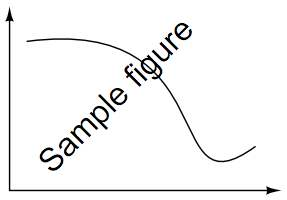
\includegraphics[width=2.5in]{samplefig}
\caption{Graph of Runtime to Number of Disks}
\label{fig:my_label}
\end{figure}

(to be added later)

\subsection{Graph of Program Memory Usage to Number of Disks}
(to find a method of keeping track of memory usage)
(to be added later)


% An example of a floating figure using the graphicx package. 
% Note that \label must occur AFTER (or within) \caption.
% For figures, \caption should occur after the \includegraphics.
% Note that IEEEtran v1.7 and later has special internal code that
% is designed to preserve the operation of \label within \caption
% even when the captionsoff option is in effect. However, because
% of issues like this, it may be the safest practice to put all your
% \label just after \caption rather than within \caption{}.
%
%\begin{figure}[!t]
%\centering
%\includegraphics[width=2.5in]{myfigure}
% where an .eps filename suffix will be assumed under latex, 
% and a .pdf suffix will be assumed for pdflatex; or what has been declared
% via \DeclareGraphicsExtensions.
%\caption{Simulation results for the network.}
%\label{fig_sim}
%\end{figure}

% Note that IEEE typically puts floats only at the top, even when this
% results in a large percentage of a column being occupied by floats.


% An example of a double column floating figure using two subfigures.
% (The subfig.sty package must be loaded for this to work.)
% The subfigure \label commands are set within each subfloat command,
% and the \label for the overall figure must come after \caption.
% \hfil is used as a separator to get equal spacing.
% Watch out that the combined width of all the subfigures on a 
% line do not exceed the text width or a line break will occur.
%
%\begin{figure*}[!t]
%\centering
%\subfloat[Case I]{\includegraphics[width=2.5in]{box}%
%\label{fig_first_case}}
%\hfil
%\subfloat[Case II]{\includegraphics[width=2.5in]{box}%
%\label{fig_second_case}}
%\caption{Simulation results for the network.}
%\label{fig_sim}
%\end{figure*}
%
\section{Results}
Discuss results here.

\section{Conclusion and Future Work}
The conclusion and discussion of what to do
going forward go here.

% references section

% can use a bibliography generated by BibTeX as a .bbl file
% BibTeX documentation can be easily obtained at:
% http://www.ctan.org/tex-archive/biblio/bibtex/contrib/doc/
% The IEEEtran BibTeX style support page is at:
% http://www.michaelshell.org/tex/ieeetran/bibtex/
\bibliographystyle{plain}
\bibliography{myrefs}
% argument is your BibTeX string definitions and bibliography database(s)
%\bibliography{IEEEabrv,../bib/paper}

\end{document}
